\documentclass[11pt,a4paper]{article} %,twocolumn
\usepackage{amsmath,amssymb,graphicx,gensymb, subcaption}
\usepackage{minted, caption} %CPP Code and captions for it 
%Sprachpaket
%\usepackage[ngerman]{babel}
%Sonderzeichen ermöglichen
\usepackage[utf8]{inputenc}
\usepackage[T1]{fontenc}
\graphicspath{{figures/}}


\begin{document}
%\twocolumn[
\begin{minipage}{1.\textwidth}
% A title page created to be used when the title should be small and not take up a whole page
\begin{titlepage}

\begin{center}
% Title
{ \huge ADI for Reaction-Diffusion Systems}

% Author

{ \emph {Lukas Strebel}} 

% Adress
{ \emph {Computational Sciences \& Engineering BSc }\\ \emph{ETH Z\"urich, Switzerland} }

{ \emph{August 3, 2015}}

\end{center}
\end{titlepage}


\end{minipage}
%]

\textit{This report is the conclusion to the project of the course High Performance Computing for Science and Engineering taught by P. Koumoutsakos and M. Troyer in the spring semester 2015.}

\section{Introduction}


\section{Gray-Scott Reaction-Diffusion - Model description} 

The Gray-Scott reaction-diffusion system \cite{gray1983autocatalytic} combines the interaction of two chemical substances and their diffusion into one set of differential equations.
The reaction between the substances U and V is described by two simple irreversible reactions:

\begin{equation} \label{chem_reac}
\begin{aligned}
	U + 2V &\rightarrow 3V \\
	V &\rightarrow P
\end{aligned}
\end{equation} 

where P is an inert product. 

\subsection{Governing Equations}

Reaction (\ref{chem_reac}) and diffusion in dimensionless units combined result in the following equations:
\begin{equation} \label{reac_diff}
\begin{aligned}
\frac{\partial u}{\partial t} &= D_u \Delta u - uv^2 + F(1-u) \\
\frac{\partial v}{\partial t} &= D_v \Delta v + uv^2 - (F+k)v
\end{aligned}
\end{equation}

where $k$ is the dimensionless rate constant of the second reaction and $F$ is the dimensionless feed rate constant. 
$D_u$ and $D_v$ are the diffusion coefficients.


\section{Discretized system}

The model is applied to a 2-dimensional domain which is discretized into a square grid with uniform, square grid cells. \\

To solve equations (\ref{reac_diff}) the reaction and diffusion are treated separately.
Diffusion is handled first and the reaction is added afterwards to the solution of the diffusion.
Since $u$ and $v$ are only coupled in the reaction their diffusion can be handled separately.

\subsection{Diffusion - Alternating Direction Implicit (ADI) method}

The general diffusion equation for a substance $\rho$ (in the Gray-Scott model u or v) is

\begin{equation} \label{gen_diff}
\frac{\partial \rho}{\partial t} = D_\rho \Delta \rho
\end{equation}

This equation could be solved by explicit or implicit methods.
However the problem with explicit methods like forward euler is instability i.e. the numerical solution will diverge from the exact solution exponentially over time.
To remain stable forward euler has a strict condition on the time step:

\begin{equation} \label{stab_cond}
	\Delta t < \frac{ \Delta x^2 \Delta y^2}{D_{\rho} ( \Delta x^2 + \Delta y^2 ) }
\end{equation}

which means for square grid cells that $ \Delta t = \Theta (h^2) $. \\

Implicit methods on the other hand are unconditionally stable but require a system of linear equations to be solved each time step. \\

The idea of the Alternating Direction Implicit (ADI) method \cite{Craig_Sneyd_1988} is to combine explicit and implicit methods in a smart way to achieve an unconditionally scheme that is second order in space and time. 

The ADI method does this by splitting each time step into two half-steps and then treating the x-direction implicitly and the y-direction explicitly in one half-step and with switched directions in the other half-step. This way each half-step consists of solving $m$ tridiagonal systems of equations, where $m$ is the size of the grid in the explicitly treated direction. The scheme looks like this: \\

First half-step:

\begin{equation} \label{adi-half1}
\rho_{i,j}^{n+\frac{1}{2}} = \rho_{i,j}^n + \frac{D_\rho \delta t}{2} \left[ \frac{\partial^2 \rho_{i,j}^{n+\frac{1}{2}}}{\partial x^2} + \frac{\partial^2 \rho_{i,j}^n}{\partial y^2} \right]
\end{equation}

Second half-step:

\begin{equation} \label{adi-half2}
\rho_{i,j}^{n+1} = \rho_{i,j}^{n+\frac{1}{2}} + \frac{D_\rho \delta t}{2} \left[ \frac{\partial^2 \rho_{i,j}^{n+\frac{1}{2}}}{\partial x^2} + \frac{\partial^2 \rho_{i,j}^{n+1}}{\partial y^2} \right]
\end{equation}

Where $i$ is the index for the grid in x-direction and $j$ is the index for the grid in y-direction. The superscript $n$ denotes the time step. \\

The second derivative is approximated using a second order central differences scheme.

\begin{equation} \label{central_differences}
\begin{aligned}
	\frac{\partial \rho_{i,j}}{\partial x^2} &= \frac{\rho_{i-1,j} - 2 \rho_{i,j} + \rho_{i+1,j}}{\Delta x^2} \\
	\frac{\partial \rho_{i,j}}{\partial y^2} &= \frac{\rho_{i,j-1} - 2 \rho_{i,j} + \rho_{i,j+1}}{\Delta y^2}
\end{aligned}
\end{equation}

For square grid cells $ \Delta x = \Delta y $.
Inserting the central differences (\ref{central_differences}) in the first half step equation (\ref{adi-half1}) results in:

\begin{equation} \label{adi_half1_complete}
\rho_{i,j}^{n+\frac{1}{2}} = \rho_{i,j}^n + \frac{D_\rho \delta t}{2} \left[ \frac{\rho_{i-1,j}^{n+\frac{1}{2}} - 2 \rho_{i,j}^{n+\frac{1}{2}} + \rho_{i+1,j}^{n+\frac{1}{2}}}{\Delta x^2} + \frac{\rho_{i-1,j}^n - 2 \rho_{i,j}^n + \rho_{i+1,j}^n}{\Delta x^2} \right]
\end{equation}

Denoting the constant coefficients as $ C = \frac{D_\rho \delta t}{2 \Delta x^2} $ and moving the implicit parts to the right hand side results in:

\begin{equation} \label{adi_half1_separated}
-C \rho_{i-1,j}^{n+\frac{1}{2}} + (1 + 2C) \rho_{i,j}^{n+\frac{1}{2}} - C \rho_{i+1,j}^{n+\frac{1}{2}} = C \rho_{i,j-1}^{n} + (1 - 2C) \rho_{i,j}^{n} - C \rho_{i,j+1}^{n} 
\end{equation}

This equation describes a tridiagonal system with the constants $-C$ on the lower and upper diagonal and the constant $ (1 + 2C) $ on the middle diagonal.
This tridiagonal system has to be solved for each row of the domain grid during the first half-step. \\

Analogously the following equation for the second half-step (\ref{adi-half2}) can be derived:

\begin{equation} \label{adi_half2_separated}
-C \rho_{i,j-1}^{n+1} + (1 + 2C) \rho_{i,j}^{n+1} - C \rho_{i,j+1}^{n+1} = C \rho_{i-1,j}^{n+\frac{1}{2}} + (1 - 2C) \rho_{i,j}^{n+\frac{1}{2}} - C \rho_{i+1,j}^{n+\frac{1}{2}}
\end{equation}

Which describes the same tridiagonal system to solve for each column of the domain grid during the second half-step.

\subsubsection{Thomas Algorithm}

One of the advantages of ADI is that it reduces the implicit part of the calculations into tridiagonal systems as described above.
This means instead of general linear system solvers a more efficient algorithm for tridiagonal systems can be used.

The Thomas algorithm is such a specialized algorithm to solve tridiagonal systems in $\mathcal O(n)$.

A general tridiagonal system for $n+1$ unknowns may be written as 

\begin{equation} \label{gen_tridiag}
a_{i} x_{i-1} + b_{i} x_{i} + c_{i} x_{i+1} = d_{i}
\end{equation}

with $a_{0} = c_{n} = 0$.

The Thomas algorithm consists of two parts, in the first part a forward sweep modifies the coefficients as follows:

\begin{equation} \label{forward_modify}
\begin{aligned}
	c'_i &=
\begin{cases}
\begin{array}{lcl}
  \cfrac{c_i}{b_i}                  & ; & i = 0 \\
  \cfrac{c_i}{b_i - a_i c'_{i - 1}} & ; & i = 1, 2, \dots, n-1 \\
\end{array}
\end{cases} \\
d'_i &=
\begin{cases}
\begin{array}{lcl}
  \cfrac{d_i}{b_i}                  & ; & i = 0 \\
  \cfrac{d_i - a_i d'_{i - 1}}{b_i - a_i c'_{i - 1}} & ; & i = 1, 2 \dots, n. \\
\end{array}
\end{cases}
\end{aligned}
\end{equation}

Where primes denote the modified coefficients.
In the second part the solution is gathered by back substition:
\begin{equation} \label{back_subst}
\begin{aligned}
	x_n &= d'_n \\
	x_i &= d'_i - c'_i\, x_{i + 1} \qquad ; \ i = n - 1, n - 2, \ldots, 0.
\end{aligned}
\end{equation}

To note is that the algorithm's forward and backward part are basically for-loops with dependencies between iterations and therefore not easily parallelizable. 

\subsection{Reaction - Forward Euler scheme}

For the reaction term of the model equations (\ref{reac_diff}) a forward Euler scheme can be applied. As noted before the reaction has to be done after the diffusion and include the solution of the diffusion equation (denoted by $\tilde u $ and $ \tilde v$)

\begin{equation} \label{reaction}
\begin{aligned}
	u_{i,j}^{n+1} &= \tilde u_{i,j}^{n+1} + \Delta t \left( - \tilde u_{i,j}^{n+1} (\tilde v_{i,j}^{n+1})^2 + F ( 1- \tilde u_{i,j}^{n+1} ) \right) \\
	v_{i,j}^{n+1} &= \tilde v_{i,j}^{n+1} + \Delta t \left( \tilde u_{i,j}^{n+1} (\tilde v_{i,j}^{n+1})^2 - (F+k) \tilde v_{i,j}^{n+1} \right)
\end{aligned}
\end{equation}

Noteworthy might be that the reaction terms (\ref{reaction}) are only dependent on the values located at the corresponding grid point i.e. they are purely local operations and require no neighborhood interactions.

\subsection{Initial conditions and constant coefficients}

A simulation domain from $ \left[ -1, 1 \right]^{2} $ was used in all implementations described in this report.
To break up the square symmetry a square in the middle of the domain contains some random noise.

\begin{equation} \label{initial_cond}
\begin{aligned}
u(x,y,0) = (1 - \chi(x,y)) + \chi(x,y) \left( \frac{1}{2} + \frac{r_{1}}{100} \right) \\
v(x,y,0) = \chi(x,y) \left( \frac{1}{4} + \frac{r_{2}}{100} \right) \\
\chi(x,y) = 
\begin{cases}
\begin{array}{ll}
  1	& \text{for } (x,y) \in [-0.2, 0.2]^{2}  \\
  0	& \text{otherwise}  \\
\end{array}	
\end{cases}
\end{aligned}
\end{equation}

where $r_{1}$ and $r_{2}$ are random numbers from a normal distribution $\mathcal{N}(0,1)$.
In our implementation we used the Mersenne-Twister random number generator provided in the C++ standard library seeded with 42 to generate these numbers.

The diffusion coefficients were defined to be $ D_{u} = 2\cdot10^{-5}$ and $ D_{v} = 1\cdot10^{-5}$ 

The parameters $F$ and $k$ were defined based on the ones described in Complex Patterns in a Simple System by J.E. Pearson \cite{Pearson_1993}.

\subsection{Boundary conditions}

Reflecting boundary conditions are used in the implementations described here.
This means that the boundaries have zero flux through their surface and everything gets reflected at them.
In terms of the previously mentioned scheme this results in a small change in the tridiagonal systems (\ref{adi_half1_separated}) and (\ref{adi_half2_separated}).
Specifically the first value on the upper diagonal $c_{0}$ and the last value on the lower diagonal $a_{n}$ have to be doubled for both the first and second half-step.


\section{Implementation}
\subsection{Serial}
\subsubsection{Outline}
Our implementation is guided by the following basic outline: \\
\begin{itemize}
\item Initialize $u$ and $v$ according to the initial conditions (\ref{initial_cond}).

\item Then for each timestep do:

	\begin{itemize}
	\item Start performance timer
	\item Perform first half-step by :
		\begin{itemize}
		\item Looping over all rows
		\item Creating the right hand side
		\item Solving the tridiagonal system with Thomas algorithm
		\end{itemize}
	\item Perform second half-step by:
		\begin{itemize}
		\item Looping over all columns
		\item Creating the right hand side
		\item Solving the tridiagonal system with Thomas algorithm
		\end{itemize}
	\item Perform reaction on each grid point
	\item Stop performance timer
	\end{itemize}
\item Calculate average time per step and standard deviation.  
\end{itemize}

\subsubsection{ADI half step implementation}

The concrete implementation of a half-step: 

\begin{center}
\begin{minted}[linenos]{c++}
 /****************** DIFFUSION (ADI) ***************************************/ 
    // perform the first half-step
    // loop over all rows
    
    // j=0
    for (int i=0; i<N_; ++i) {
        uRhs[i] = U(i,0) + uCoeff * (U(i,1) - U(i,0));
        vRhs[i] = V(i,0) + vCoeff * (V(i,1) - V(i,0));
    }
    TriDiagMatrixSolver::solve(N_, matU1_, uRhs, &UHALF(0,0), 1);
    TriDiagMatrixSolver::solve(N_, matV1_, vRhs, &VHALF(0,0), 1);
    
    // inner grid points
    for (int j=1; j<N_-1; ++j) {
        // create right-hand side of the systems
        for (int i=0; i<N_; ++i) {
            uRhs[i] = U(i,j) + uCoeff * (U(i,j+1) - 2.*U(i,j) + U(i,j-1));
            vRhs[i] = V(i,j) + vCoeff * (V(i,j+1) - 2.*V(i,j) + V(i,j-1));
        }
        
        TriDiagMatrixSolver::solve(N_, matU1_, uRhs, &UHALF(0,j), 1);
        TriDiagMatrixSolver::solve(N_, matV1_, vRhs, &VHALF(0,j), 1);
    }
    
    // j=N_-1
    for (int i=0; i<N_; ++i) {
        uRhs[i] = U(i,N_-1) + uCoeff * (- U(i,N_-1) + U(i,N_-2));
        vRhs[i] = V(i,N_-1) + vCoeff * (- V(i,N_-1) + V(i,N_-2));
    }
    TriDiagMatrixSolver::solve(N_, matU1_, uRhs, &UHALF(0,N_-1), 1);
    TriDiagMatrixSolver::solve(N_, matV1_, vRhs, &VHALF(0,N_-1), 1);
\end{minted}
\captionof{listing}{Implementation of first half-step, second half-step is done analogously except the role of i and j are switched. \label{lst:ADI_implementation}} 
\end{center}

The values of $u$ and $v$ are stored row wise in a \texttt{std::vector<double>}.
For ease of use preprocessor \texttt{\#define} directives are used to access $u$ and $v$ via \texttt{ U(i,j) } or \texttt{ V(i,j)} respectively.
The boundary rows in the first half-step and the boundary columns in the second half-step have to be done outside of the main loop because of their different dependencies on the neighbouring cells.
\texttt{matU1} and \texttt{matV1} refer to the tridiagonal system described in the ADI section (\ref{adi_half1_separated}, \ref{adi_half2_separated}).
We encapsulated these tridiagonal system into their own class that stores the diagonals each in a \texttt{std::vector<double>} and provides access to them. Also that way they can be passed to the solver as a single object. 

\subsubsection{Thomas algorithm implementation}

\texttt{TriDiagMatrixSolver::solve(...)} in listing \ref{lst:ADI_implementation} is our implementation of the Thomas algorithm, which is a modified version of the implementation found on Wikipedia in April 2014 \cite{wiki:thomas-alg}. 

\begin{center}
\begin{minted}[linenos]{c++}
void TriDiagMatrixSolver::solve(int n, const TriDiagMatrix& mat, 
const std::vector<double>& rhs, double *result, unsigned int inc)
{
   
    std::vector<double> a = mat.getL(); // lower diagonal, indexed 1..n-1
    std::vector<double> b = mat.getM(); // main diagonal, indexed 0..n-1
    std::vector<double> c = mat.getU(); // upper diagonal, indexed 0..n-2
    
    
    n--; // since we start from x_0 (not x_1) (n now denotes the max index)
    c[0] /= b[0];
    
    std::vector<double> r(rhs);
    r[0] /= b[0];
    
    double tmp;

    for (int i=1; i<n; ++i) {
        tmp = b[i] - a[i]*c[i-1];
        c[i] /= tmp;
        r[i] = (r[i] - a[i]*r[i-1]) / tmp;
    }

    *(result + n*inc) = (r[n] - a[n]*r[n-1]) / (b[n] - a[n]*c[n-1]);

    for (int i=n-1; i>=0; --i) {
        *(result + i*inc) = r[i] - c[i] * (*(result + (i+1)*inc));
    }
}
\end{minted}
\captionof{listing}{Implementation of Thomas algorithm. \label{lst:Thomas_implementation}} 
\end{center}
In order to use the same function for each row/column and for both half-steps we use the \texttt{double *result} argument as the pointer to the first element of the row/column for which the function was called and the \texttt{unsigned int inc} argument to distinguish between row-wise access (for the first half-step \texttt{inc} = 1 and column-wise access for the second half-step \texttt{inc} = N.

\subsubsection{Implementation of reaction}

After the second half-step is done the reaction can be performed.
\begin{center}
\begin{minted}[linenos]{c++}
    /****************** REACTION **********************************************/

    double tmp;
    for (int i=0; i<N_; ++i) {
        for (int j=0; j<N_; ++j) {
            tmp = U(i,j);
            U(i,j) += dt_ * ( -U(i,j)*V(i,j)*V(i,j) + F_*(1.-U(i,j)) );
            V(i,j) += dt_ * ( tmp*V(i,j)*V(i,j) - (F_+k_)*V(i,j) );
        }
    }
\end{minted}
\captionof{listing}{Implementation of reaction. \label{lst:reaction_implementation}} 
\end{center}

As mentioned before the reaction equation (\ref{reaction}) has to be done on each gridpoint locally and doesn't depend on any neighbours.

\subsection{OpenMP implementation}

Our parallelization with OpenMP consists of three parallel regions, one for each half-step to parallelize the loop over the inner grid points and one more to parallelize the reaction across the whole grid.

\begin{center}
\begin{minted}[linenos]{c++}
// inner grid points

#pragma omp parallel num_threads(nthreads_)
    { // PARALLEL REGION BEGIN
    // right hand sides for u and for v
    std::vector<double> puRhs(N_);
    std::vector<double> pvRhs(N_);

#pragma omp for
    for (int j=1; j<N_-1; ++j) {
        // create right-hand side of the systems
        for (int i=0; i<N_; ++i) {
            puRhs[i] = U(i,j) + uCoeff * (U(i,j+1) - 2.*U(i,j) + U(i,j-1));
            pvRhs[i] = V(i,j) + vCoeff * (V(i,j+1) - 2.*V(i,j) + V(i,j-1));
        }
        
        TriDiagMatrixSolver::solve(N_, matU1_, puRhs, &UHALF(0,j), 1);
        TriDiagMatrixSolver::solve(N_, matV1_, pvRhs, &VHALF(0,j), 1);
    }
    } // PARALLEL REGION END
\end{minted}
\captionof{listing}{Parallelization of the inner grid points in the first ADI half-step with OpenMP (second half-step done analogously). \label{lst:omp_halfstep}} 
\end{center}

As shown in listing \ref{lst:omp_halfstep} we parallelize the outer loop in the half-steps as they have only read-dependencies on the other rows (first half-step) / columns (second half-step).
Each thread declares its own private right hand side inside the parallel region and writes the result of the tridiagonal solver in a region of the result vector that no other thread reads or writes to. 
This is due to the fact that the end of the parallel region after the first half-step represents a implicit barrier before the parallel region of the second half-step starts.
All other variables are read-only and can therefore be safely shared by all threads.

\begin{center}
\begin{minted}[linenos]{c++}
#pragma omp parallel num_threads(nthreads_)
    { // PARALLEL REGION BEGIN
    double tmp;
#pragma omp for collapse(2)
    for (int i=0; i<N_; ++i) {
        for (int j=0; j<N_; ++j) {
            tmp = U(i,j);
            U(i,j) += dt_ * ( -tmp*V(i,j)*V(i,j) + F_*(1.-tmp) );
            V(i,j) += dt_ * ( tmp*V(i,j)*V(i,j) - (F_+k_)*V(i,j) );
        }
    }
    } // PARALLEL REGION END
\end{minted}
\captionof{listing}{Parallelization of the reaction with OpenMP \label{lst:omp_reaction}} 
\end{center}

Since the reaction as mentioned before is local to each grid point the parallelization of the two loops can be done together with the \texttt{collapse} option of the pragma omp for.

\subsection{MPI implementation}

For the parallelization with MPI on distributed memory the domain needs to be split equally among the processors.
Because the first half step requires a processor to have full rows the simplest way to distribute the grid is block row-wise.
This way each processor gets a set of neighbouring rows and can do its job on the local, inner rows without any communications with the other processors.

For the top and bottom row of each processor's local grid read access to one additional row of a neighbouring processor bottom or top row respectively is required.
Since we work on a Cartesian grid we can use the MPI Cartesian topology to easily find the neighbours of a processors using the \texttt{MPI\_Cart\_shift} function.
To do the local boundaries efficiently ghost rows are used and communicated using non-blocking methods so that the communication and the computation of the inner grid cells can be overlapped as shown in listing (\ref{lst:communication}).

\begin{center}
\begin{minted}[linenos]{c++}
// exchange boundaries
    if (world.coord_x % 2 == 0) {       
MPI_Isend(&u_[(Nx_loc)*(Ny_loc)],   1, bottom_boundary, world.bottom_proc,
 TAG, cart_comm, &request[0]);
MPI_Irecv(&u_[(Nx_loc+1)*(Ny_loc)], 1, bottom_boundary, world.bottom_proc,
 TAG, cart_comm, &request[1]);
MPI_Isend(&u_[(Ny_loc)],            1, top_boundary,    world.top_proc, 
   TAG, cart_comm, &request[2]);
MPI_Irecv(&u_[0],                   1, top_boundary,    world.top_proc,  
 TAG, cart_comm, &request[3]);
        // exactly the same for v, omitted here
    }
    else {      
MPI_Irecv(&u_[0],                   1, top_boundary,    world.top_proc,  
  TAG, cart_comm, &request[0]);
MPI_Isend(&u_[(Ny_loc)],            1, top_boundary,    world.top_proc,  
  TAG, cart_comm, &request[1]);
MPI_Irecv(&u_[(Nx_loc+1)*(Ny_loc)], 1, bottom_boundary, world.bottom_proc,
 TAG, cart_comm, &request[2]);
MPI_Isend(&u_[(Nx_loc)*(Ny_loc)],   1, bottom_boundary, world.bottom_proc,
 TAG, cart_comm, &request[3]);
        // exactly the same for v, omitted here
    }

	// Do inner grid cells computations
\end{minted}
\captionof{listing}{Communication of ghost cells before each ADI half-step\label{lst:communication}} 
\end{center}

After the local, inner grid cells are calculated the processors have to wait until the non-blocking communications are done and then the local boundaries can be computed.
Special care has to be taken for the processors that are on the global grid boundaries which have to do the boundary calculations in the way described before (for example in listing (\ref{lst:ADI_implementation})).
\\
The thus far described MPI implementation works for the first half-step.
The second half-step however requires each processor to have full columns and therefore we need to transpose the grid beforehand.

This means each processor needs to split its set of rows into blocks with the width of each block equal to the number of rows each processor has in its row block.
These blocks then correspond to the grid points that have to be sent to the same processor.
The blocks are sent using \texttt{MPI\_Alltoall} but they still need to be transposed.
To do the transpose we have two different approaches.

The first approach receives the blocks and transposes each block locally according to listing (\ref{lst:transpose_local}).

\begin{center}
\begin{minted}[linenos]{c++}
        MPI_Alltoall(&uTemp[Ny_loc], 1, block_resized_send, 
&u_[Ny_loc], 1, block_resized_send, MPI_COMM_WORLD);
        MPI_Alltoall(&vTemp[Ny_loc], 1, block_resized_send, 
&v_[Ny_loc], 1, block_resized_send, MPI_COMM_WORLD);
        
        // locally transpose blocks
        // loop over blocks
        int ind1, ind2;
        for (int b=0; b<Nb_loc; ++b) {
            for (int i=0; i<Nx_loc; ++i) {
                for (int j=0; j<i; ++j) {
                    ind1 = (i+1)*Ny_loc + j + b*Nx_loc; 
	// regular index + offset of block
                    ind2 = (j+1)*Ny_loc + i + b*Nx_loc; 
	// switch i and j
                    
                    std::swap(u_[ind1], u_[ind2]);
                    std::swap(v_[ind1], v_[ind2]);
                }
            }
        }
\end{minted}
\captionof{listing}{Approach one to transpose the grid based on \texttt{MPI\_Alltoall} with one send/receive data type and a locally done transpose of each block. \label{lst:transpose_local}} 
\end{center}

The second approach changes the receive data type in such a way that is the transpose of the sent data type see listing (\ref{lst:transpose_datatypes}).

\begin{center}
\begin{minted}[linenos]{c++}
    // build datatypes for transpose
    MPI_Datatype block_send, block_col, block_recv;
    
    // send data type

    // define the sizes for the blocks
    // size of the whole region the processor handles
    int sizes[2]    = {Nx_loc, Ny_loc};
    // size of sub-region (square) / blocks to be sent for transpose
    int subsizes[2] = {Nx_loc, Nx_loc}; 
    // where does the first subarray begin (which index)
    int starts[2]   = {0,0};            
    
    // creating the blocks
    MPI_Type_create_subarray(2, sizes, subsizes, starts, 
MPI_ORDER_C, MPI_DOUBLE, &block_send);
    MPI_Type_commit(&block_send);

    // resize -> make contiguous
    MPI_Type_create_resized(block_send, 0, Nx_loc*sizeof(double),
 &block_resized_send);
    MPI_Type_free(&block_send);
    MPI_Type_commit(&block_resized_send);
    
    
    // receive datatype ( for 2nd approach of transpose)

    // define a row of the transposed (receive) block 
    // as vector with a stride of the length of the old row
    // this way each element of an old column will be in the same new row 
    // and in the correct order
    MPI_Type_vector(Nx_loc, 1, Ny_loc, MPI_DOUBLE, &block_col);
    MPI_Type_commit(&block_col);

    // combine the new rows into a block
    MPI_Type_hvector(Nx_loc, 1, sizeof(double), block_col, &block_recv);
    MPI_Type_free(&block_col);
    MPI_Type_commit(&block_recv);

    // resize data structure, so that it is contiguous (for alltoall)
    MPI_Type_create_resized(block_recv, 0, sizeof(double),
 &block_resized_recv);
    MPI_Type_free(&block_recv);
    MPI_Type_commit(&block_resized_recv);

\end{minted}
\captionof{listing}{. \label{lst:transpose_datatypes}} 
\end{center}

With a receive type defined like described the transpose after each half-step is done in a single call to \texttt{MPI\_Alltoall} for $u$ and one for $v$. (See listing (\ref{lst:transpose_alltoall}))

\begin{center}
\begin{minted}[linenos]{c++}
        // after half-step is done:

        MPI_Alltoall(&uTemp[Ny_loc], 1, block_resized_send, 
&u_[Ny_loc], 1, block_resized_recv, MPI_COMM_WORLD);
        MPI_Alltoall(&vTemp[Ny_loc], 1, block_resized_send, 
&v_[Ny_loc], 1, block_resized_recv, MPI_COMM_WORLD);
	
	// ready for next half-step or reaction
\end{minted}
\captionof{listing}{. \label{lst:transpose_alltoall}} 
\end{center}

After the second half-step including the transposing of the grid is done, each processor can perform the reaction on its own grid points.

\subsection{Hybrid OpenMP + MPI implementation}

Our hybrid version combines OpenMP and MPI by enhancing the pure MPI version with OpenMP threads to do the inner grid cells of each processor in parallel like the pure OpenMP version does it.
OpenMP threads are also used to do reaction as well as the local transpose in parallel (if approach one is used and not approach two).

\section{Results}
\subsection{Correctness}

To see if our implementations produce the expected results we implemented a visualization using OpenGL to display the evolution of the concentration of $u$ during the time stepping. 

Since some patterns take a lot of time steps to develop we later used LodePNG \cite{lodepng} as a image encoder to save an image of the concentration of $u$ at the end of simulation time only.

We tried to recreate the same patterns Pearson  got in his paper \cite{Pearson_1993}, the results can be seen in Figure (\ref{fig:patterns}).


\begin{figure}
	
	\captionsetup{format=hang}
	\begin{subfigure}{0.15\textwidth}
		\centering
		\includegraphics[width=\textwidth]{patterns/{alpha_k_0.046_F_0.007_step_100000}.png}
		\caption{\tiny Pattern $\alpha$\\$F=0.007$\\$k=0.046$}
		\label{fig:pattern-alpha}
	\end{subfigure}
	\quad
	\begin{subfigure}{0.15\textwidth}
		\centering
		\includegraphics[width=\textwidth]{patterns/{beta_k_0.046_F_0.020_step_100000}.png}
		\caption{\tiny Pattern $\beta$\\$F=0.020$\\$k=0.046$}
		\label{fig:pattern-beta}
	\end{subfigure}
	\quad
	\begin{subfigure}{0.15\textwidth}
		\centering
		\includegraphics[width=\textwidth]{patterns/{gamma_k_0.055_F_0.024_step_100000}.png}
		\caption{\tiny Pattern $\gamma$\\$F=0.024$\\$k=0.055$}
		\label{fig:pattern-gamma}
	\end{subfigure}
	\quad
	\begin{subfigure}{0.15\textwidth}
		\centering
		\includegraphics[width=\textwidth]{patterns/{delta_k_0.055_F_0.030_step_100000}.png}
		\caption{\tiny Pattern $\delta$\\$F=0.030$\\$k=0.055$}
		\label{fig:pattern-delta}
	\end{subfigure}
	
	\begin{subfigure}{0.15\textwidth}
		\centering
		\includegraphics[width=\textwidth]{patterns/{epsilon_k_0.055_F_0.019_step_100000}.png}
		\caption{\tiny Pattern $\epsilon$\\$F=0.019$\\$k=0.055$}
		\label{fig:pattern-epsilon}
	\end{subfigure}
	\quad
	\begin{subfigure}{0.15\textwidth}
		\centering
		\includegraphics[width=\textwidth]{patterns/{xi_k_0.061_F_0.024_step_100000}.png}
		\caption{\tiny Pattern $\zeta$\\$F=0.024$\\$k=0.061$}
		\label{fig:pattern-zeta}
	\end{subfigure}
	\quad
	\begin{subfigure}{0.15\textwidth}
		\centering
		\includegraphics[width=\textwidth]{patterns/{eta_k_0.063_F_0.035_step_100000}.png}
		\caption{\tiny Pattern $\eta$\\$F=0.035$\\$k=0.063$}
		\label{fig:pattern-eta}
	\end{subfigure}
	\quad
	\begin{subfigure}{0.15\textwidth}
		\centering
		\includegraphics[width=\textwidth]{patterns/{theta_k_0.060_F_0.042_step_100000}.png}
		\caption{\tiny Pattern $\theta$\\$F=0.042$\\$k=0.060$}
		\label{fig:pattern-theta}
	\end{subfigure}
	
	\begin{subfigure}{0.15\textwidth}
		\centering
		\includegraphics[width=\textwidth]{patterns/{iota_k_0.060_F_0.050_step_100000}.png}
		\caption{\tiny Pattern $\iota$\\$F=0.050$\\$k=0.060$}
		\label{fig:pattern-iota}
	\end{subfigure}
	\quad
	\begin{subfigure}{0.15\textwidth}
		\centering
		\includegraphics[width=\textwidth]{patterns/{kappa_k_0.063_F_0.050_step_100000}.png}
		\caption{\tiny Pattern $\kappa$\\$F=0.050$\\$k=0.063$}
		\label{fig:pattern-kappa}
	\end{subfigure}
	\quad
	\begin{subfigure}{0.15\textwidth}
		\centering
		\includegraphics[width=\textwidth]{patterns/{lambda_k_0.065_F_0.040_step_100000}.png}
		\caption{\tiny Pattern $\lambda$\\$F=0.040$\\$k=0.065$}
		\label{fig:pattern-lambda}
	\end{subfigure}
	\quad
	\begin{subfigure}{0.15\textwidth}
		\centering
		\includegraphics[width=\textwidth]{patterns/{mu_k_0.065_F_0.050_step_100000}.png}
		\caption{\tiny Pattern $\mu$\\$F=0.050$\\$k=0.065$}
		\label{fig:pattern-mu}
	\end{subfigure}
	\caption{Concentration of $u$ visualized after $10^5$ steps}
	\label{fig:patterns}
\end{figure}

\subsection{Performance}
\subsubsection{Test environment}

To test the performance of our implementations we were allowed to use the Piz Daint supercomputer of the Swiss National Supercomputing Centre (CSCS).
The Piz Daint is a Cray XC30 system and has 5272 compute nodes in total.

Each compute node features an Intel Xeon E5-2670 "Sandybridge" CPU running at a nominal frequency of 2.6 GHz with 8 physical cores per CPU, which can run 2 "hyperthread" hardware threads on each core and has 32 GB of memory.

Each node also features a Nvidia Tesla K20x "Kepler" GPU which sadly we didn't take advantage of in this project.

\subsubsection{System size scaling comparison}

In all the following measurements we took the time of each step in a simulation over $10^{3}$ steps and averaged them. 
Also shown in each figure are the standard deviations of the measurements as error bars (which in all cases are barely visible).

In figure (\ref{fig:system_size_scaling}) we compared how the different implementations scale with the system size.
For the serial implementation we took these measurements for a non vectorized as well as a version compiled with \texttt{g++ -ftree-vectorize} but we observed no significant difference between the two and therefore the vectorized version was omitted.

Not suprisingly the hybrid MPI + OpenMP version shows the best overall scaling with system size.
However for very large systems the hybrid version approaches the pure MPI version, which could be seen as a hint that the communication between nodes and not how fast each node does its computation becomes the limiting factor.

\begin{figure}
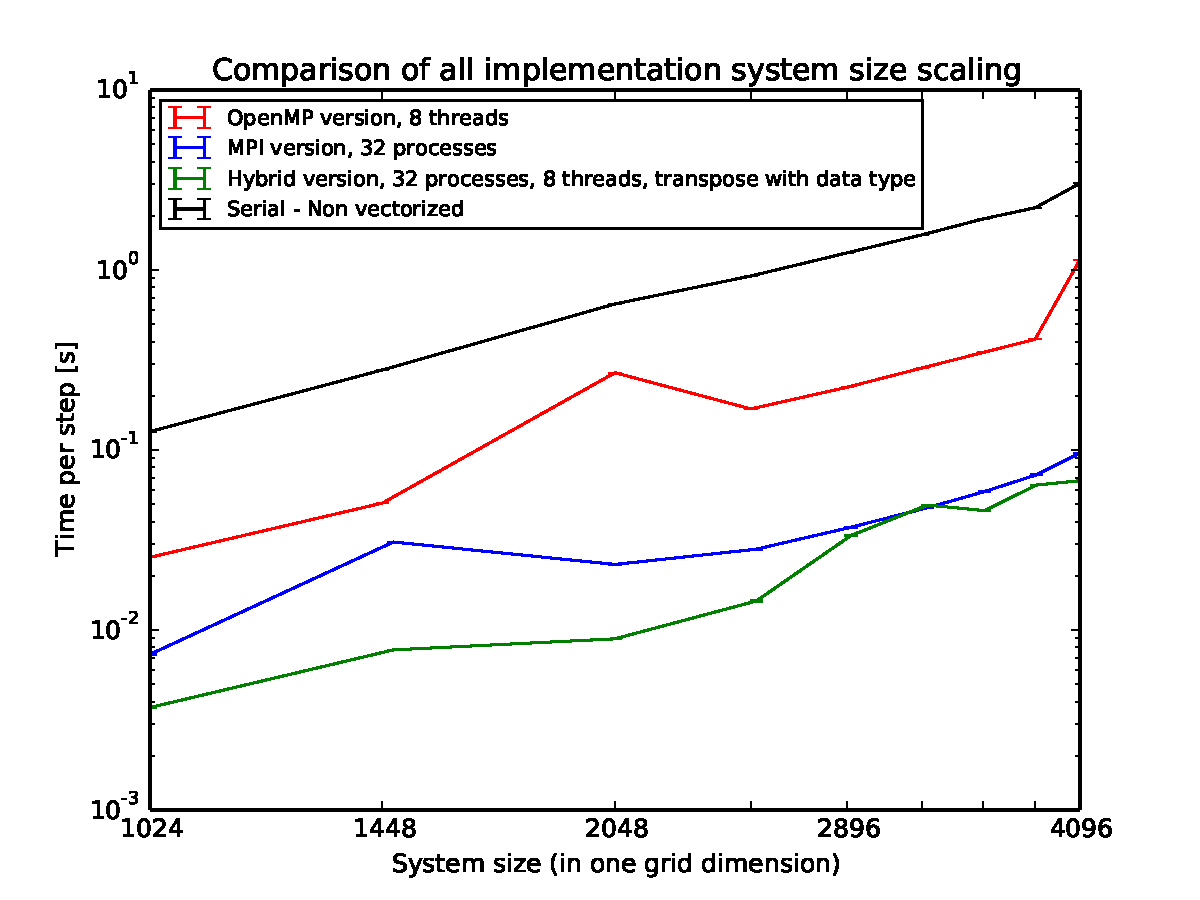
\includegraphics[width=\textwidth]{comparison_system_size_scaling.pdf}
\caption{Comparison of the various implementations in regard to their scaling with system size}
\label{fig:system_size_scaling}
\end{figure}

\subsubsection{Different transpose approaches}

In figure (\ref{fig:transpose_system_size_scaling}) we looked at the performance of our two different approaches to the transpose.
We used the MPI version with 32 MPI processes and found that both approaches scale quite similarly.


\begin{figure}
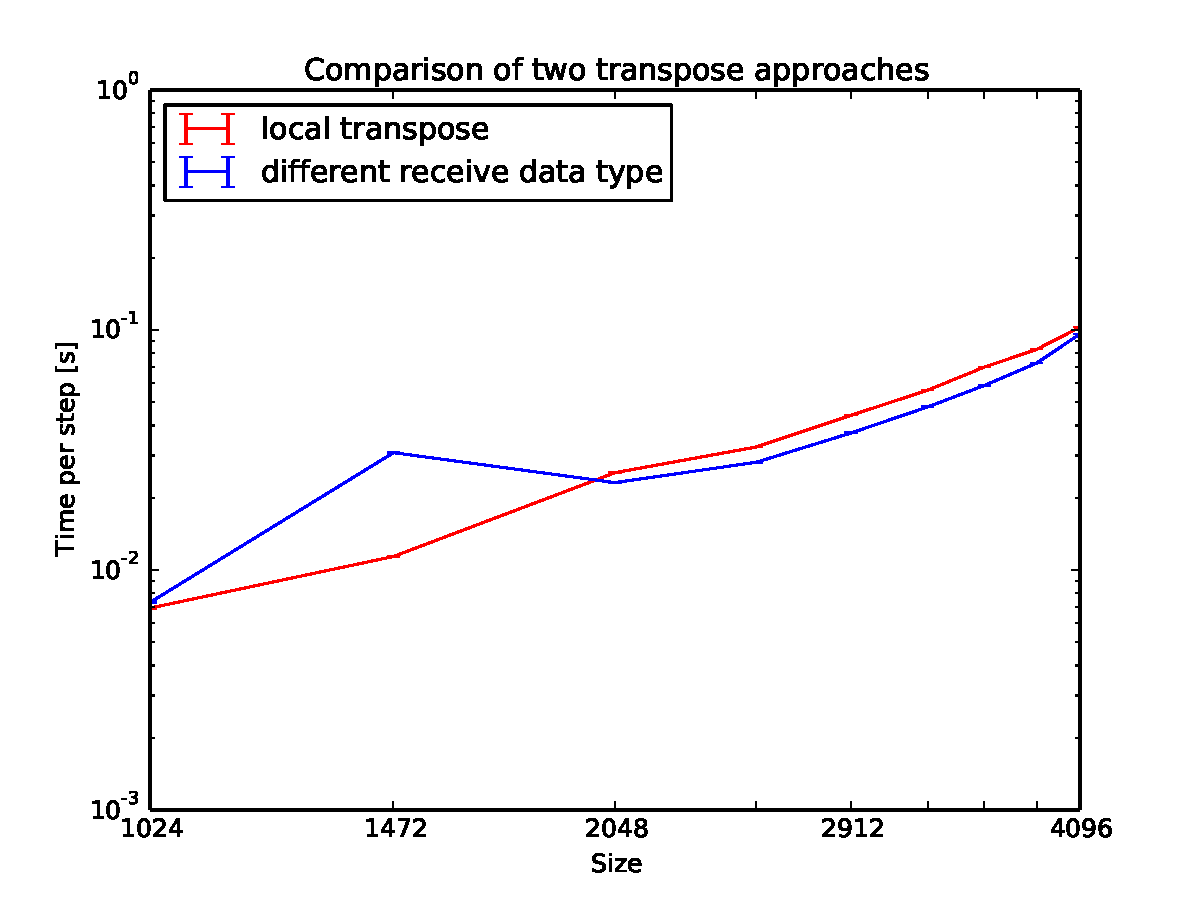
\includegraphics[width=\textwidth]{mpi_transpose_32.pdf}
\caption{Comparison of the two approaches to the transpose after each half-step in the MPI versions with regards to their scaling with system size.}
\label{fig:transpose_system_size_scaling}
\end{figure}

\subsubsection{Strong scaling}

We also wanted to see how our implementation scaled without increasing the system size i.e. what the strong scaling plots look like.

First up the OpenMP version seen in figure (\ref{fig:omp_strong_scaling}) shows quite good speed up for the smaller system sizes but stagnates around 8 threads for all system sizes.
This stagnation seems to be reasonable considering that in our test environment after 8 threads hyperthreading sets in.

We also think that we could have improved the performance of the OpenMP (and indirectly the hybrid version) by making it NUMA aware for instance by using a first-touch policy for our $u$ and $v$ vector. \\

\begin{figure}
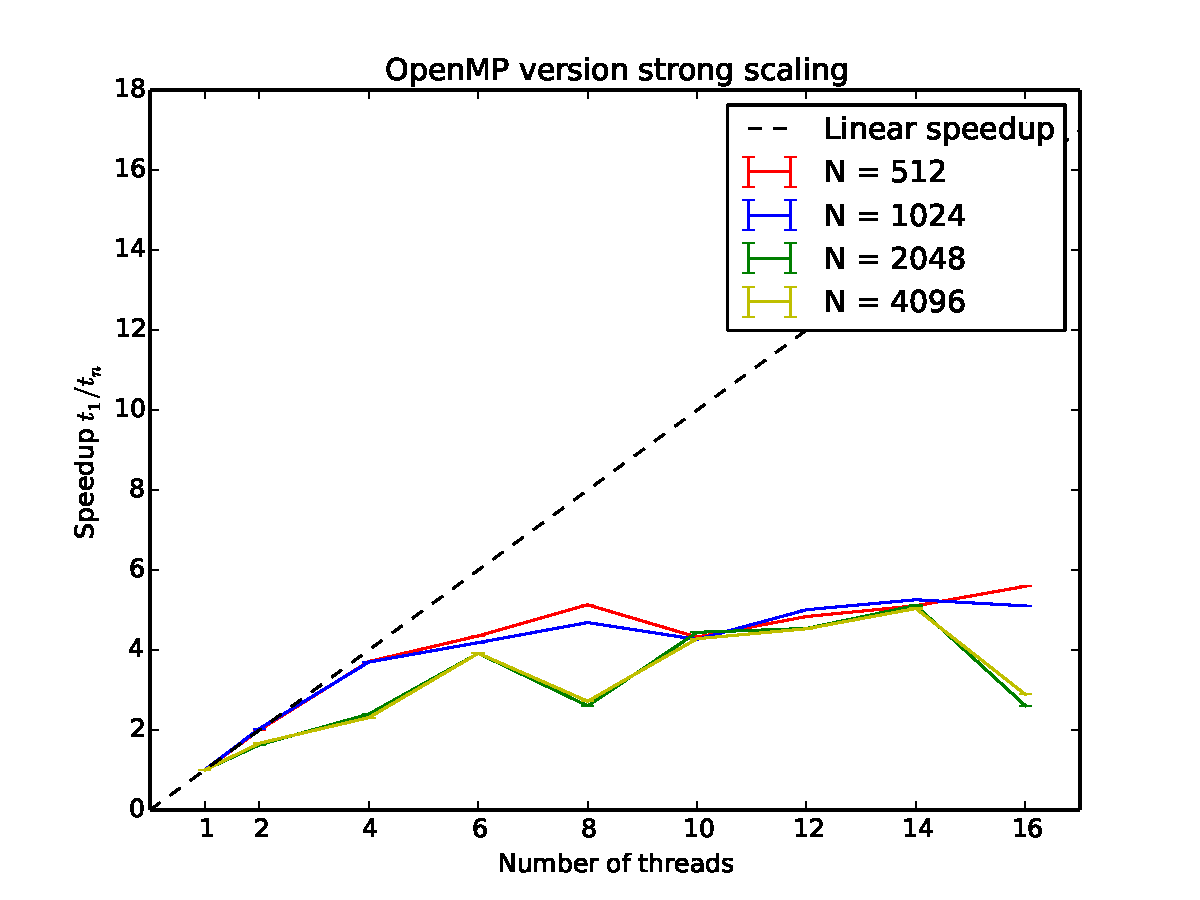
\includegraphics[width=\textwidth]{omp_strong_scaling.pdf}
\caption{Strong scaling plot of the OpenMP implementation.}
\label{fig:omp_strong_scaling}
\end{figure}

The speed up of the pure MPI version (see figure (\ref{fig:mpi_strong_scaling})) on the other hand depends strongly on the size of the system.
For smaller systems the speed up stagnates around 16 processes while for the larger systems almost linear speed up is achieved up to 128 processes. \\

\begin{figure}
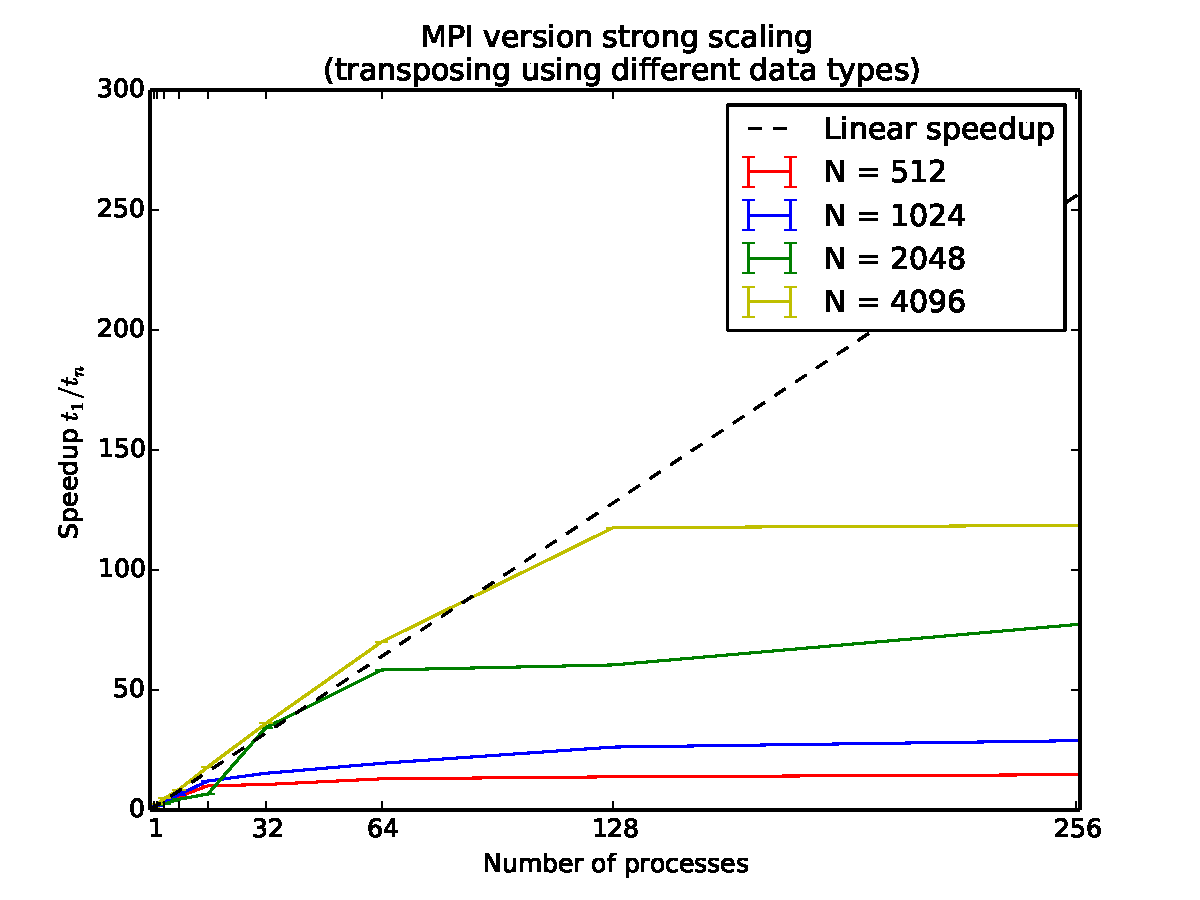
\includegraphics[width=\textwidth]{mpi_data_strong_scaling.pdf}
\caption{Strong scaling plot of the MPI implementation.}
\label{fig:mpi_strong_scaling}
\end{figure}

Lastly the strong scaling of the hybrid version (seen in figure (\ref{fig:hybrid_strong_scaling})) shows similar structure as the pure MPI one.
However for the larger systems it also shows super linear scaling up to 128 processes with 8 OpenMP threads each. \\

\begin{figure}
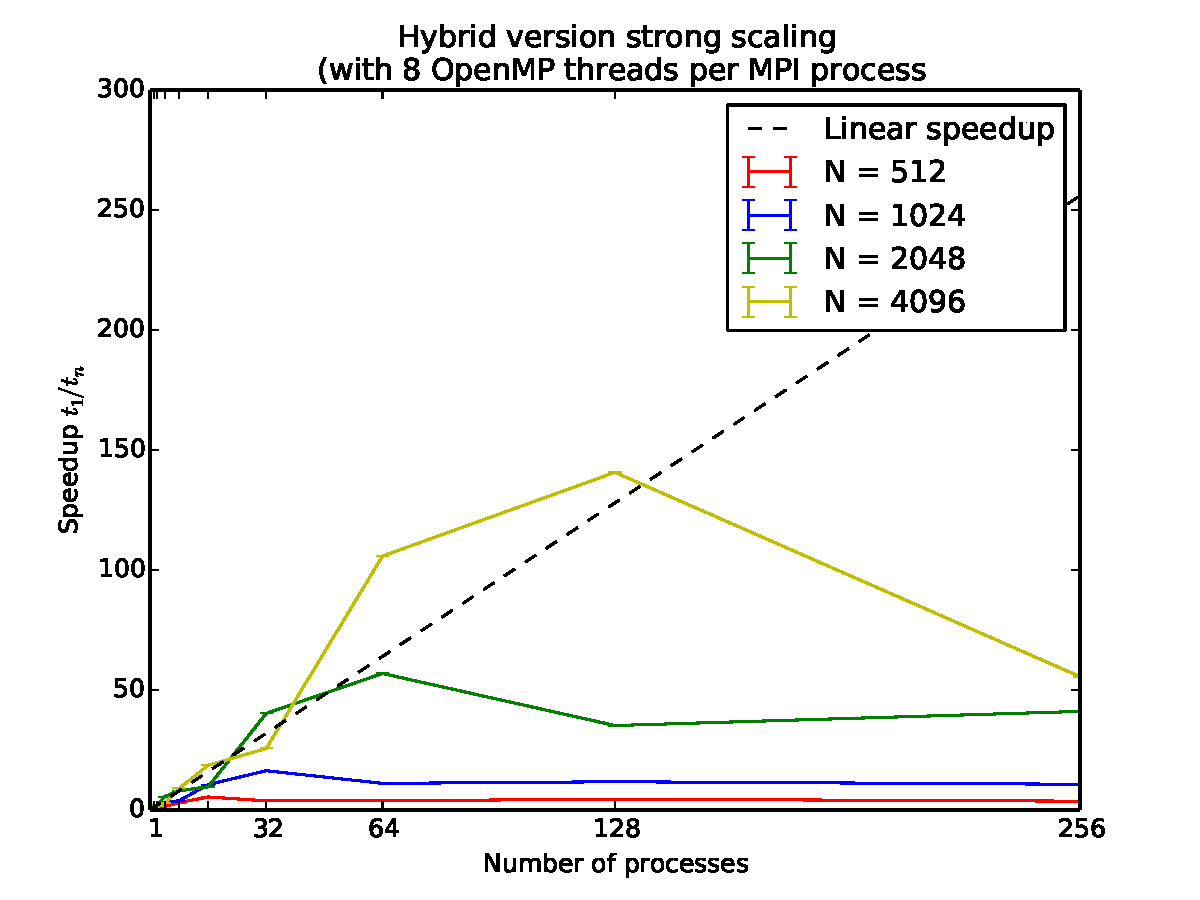
\includegraphics[width=\textwidth]{hybrid_strong_scaling.pdf}
\caption{Strong scaling plot of the Hybrid MPI+OpenMP implementation.}
\label{fig:hybrid_strong_scaling}
\end{figure}

We also experimented around with the number of OpenMP threads in the hybrid version. (seen in figure (\ref{fig:hybrid_omp_comparison}))
We found that while it can make a difference in smaller systems and when not using many MPI processes, for the larger systems and when using more MPI processes the difference the number of OpenMP threads makes becomes less and less important to the overall scaling. \\

\begin{figure}[htp]
\centering
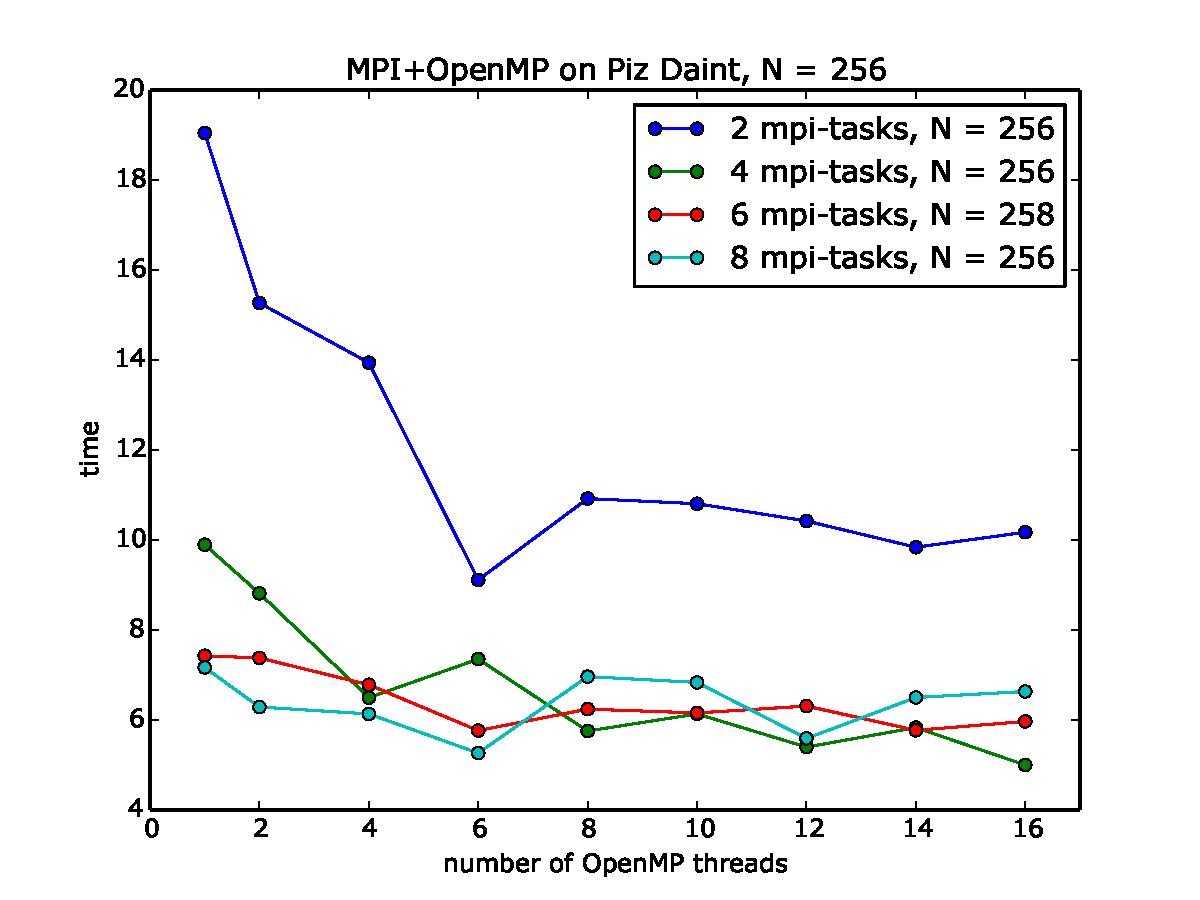
\includegraphics[width=.5\textwidth]{hybrid_omp_compare_256.pdf}\hfill
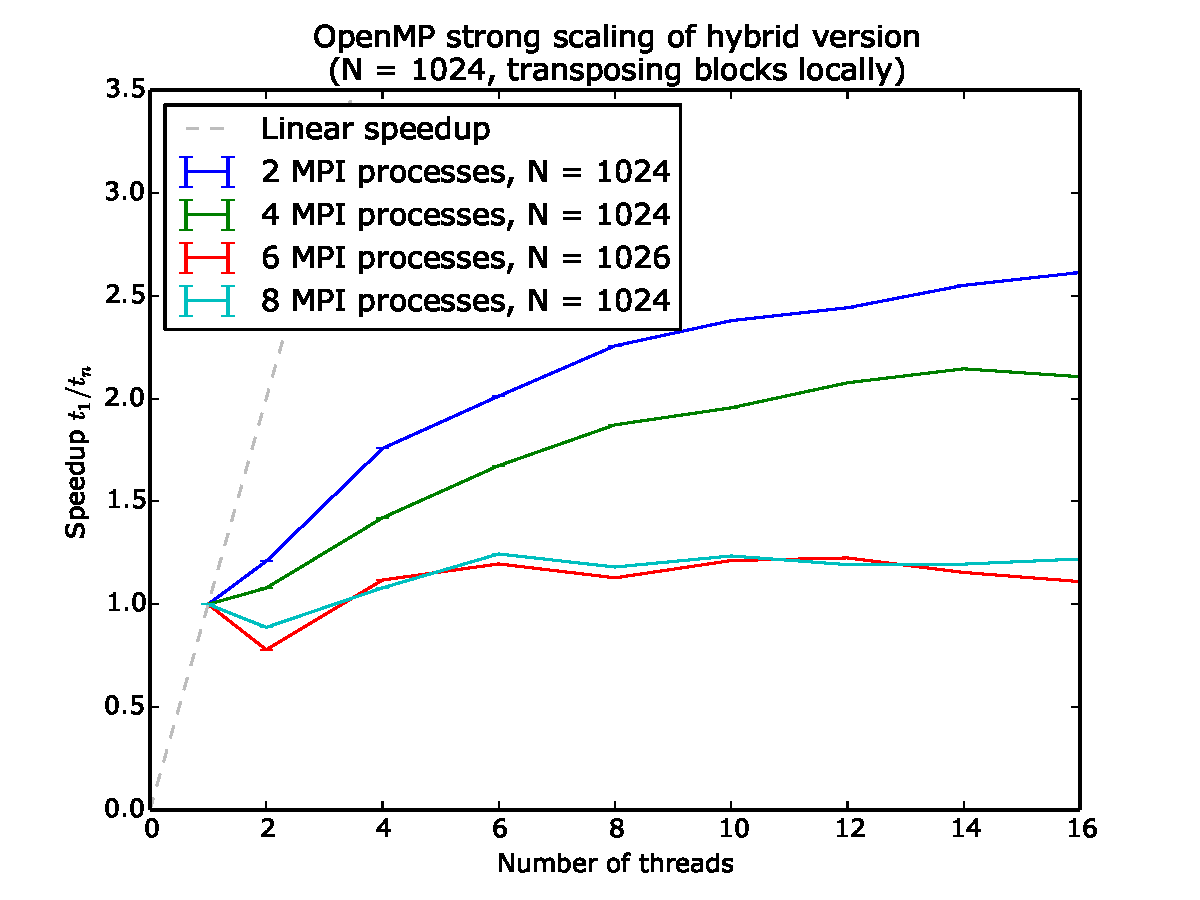
\includegraphics[width=.5\textwidth]{hybrid_omp_compare_1024.pdf}
\caption{The Difference the number of OpenMP threads makes in the hybrid version for two example system sizes.}
\label{fig:hybrid_omp_comparison}
\end{figure}

\subsubsection{Energy consumption}

During one of the strong scaling experiments for the pure MPI version we looked at the energy consumption reported by the Piz Daint system.
\\
The results are summarized in table (\ref{table:energy}), as can be expected the energy consumption varies due to how long the simulation takes and on how many nodes are used.
Of course both of these factors depend on the number of processes used.
In our case we can see a sharp decline in power consumption in the region we see good speed up in figure (\ref{fig:mpi_strong_scaling}) and then a strong increase in power consumption, when the speed up stagnates.

\begin{table}[h] \label{table:energy}
\begin{tabular}{| l | l | l | l | l | l | l | l | l | l |}
\hline
MPI processes & 1 & 2 & 4 & 8 & 16 & 32 & 64 & 128 & 256 \\ \hline
Energy [in joule] & 66982 & 30434 & 36037 & 25470 & 34324 & 13861 & 17199 & 32931 & 52283 \\ \hline
\end{tabular}
\caption{Energy consumption during strong scaling experiments.}
\end{table}


\section{Summary}

%\begin{center}
%\begin{minted}[linenos]{c++}

%\end{minted}
%\captionof{listing}{. \label{lst:}} 
%\end{center}

\bibliographystyle 	{IEEEbib} 
\bibliography 		{bibl_conf}

\end{document}

